\section{Introduction}
Reconfiguration of consensus protocol is not a new topic, it has been studies for decades and has more and more use cases in recent blockchain
area.

We'll present our mechanism to support reconfiguration of \LBFT in section \ref{mechanism}, and discuss the approches we considered and
comparison between them in section \ref{alternatives}, finally we'll give the correctness argument for all approaches in section \ref{correctness}.

At the high level, reconfiguration is under the authority of the current set of validators and operates via reconfig-transactions embedded inside the normal chain of transactions.
The chain continues beyond the reconfiguration transaction just like normal transactions, and the node should use the on-chain configuration to
spawn \LBFT instance. Genesis transaction is the first reconfiguration transaction and defines the configuration for the first \LBFT instance.

Epoch is the counter for the on-chain configurations, it's bumped after reconfiguration transactions. \LBFT instance is constructed with configuration
including epoch, ledger state, validator set etc. and initializes its internal state such as setting round to 0, generating genesis block for block store
etc. Blocks in different epochs are not chained and are internal to each \LBFT instance, but the underlying ledger state(chain of transactions) are continued.

\begin{figure}[ht]
	\centering
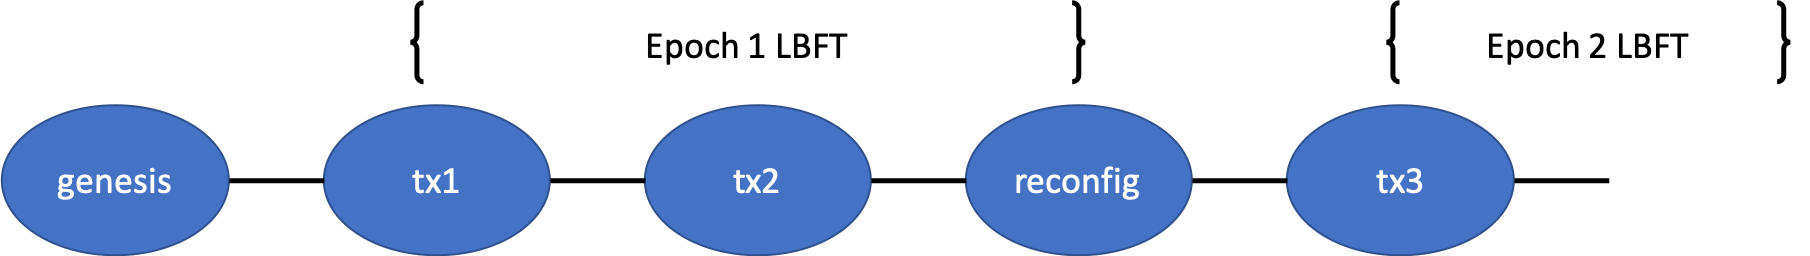
\includegraphics[scale=.45]{figures/introduction.png}
\caption{reconfiguraiton with multi LBFT instances}
\end{figure}
